\documentclass[aspectratio=169,11pt]{beamer}

% Theme and colors
\usetheme{Madrid}
\usecolortheme{whale}
\setbeamertemplate{navigation symbols}{}
\setbeamertemplate{footline}[frame number]

% Packages
\usepackage[utf8]{inputenc}
\usepackage[T1]{fontenc}
\usepackage{graphicx}
\usepackage{booktabs}
\usepackage{amsmath}
\usepackage{hyperref}
\usepackage{tikz}
\usetikzlibrary{shapes,arrows,positioning,calc,fit,backgrounds}
\usepackage{siunitx}
\usepackage{xcolor}
\usepackage{array}

% Title information
\title[EECE5155 -- Module 8]{Data Analytics for IoT}
\subtitle{Module 8: From Raw Data to Actionable Intelligence}
\author{Eduardo Baena}
\date{Spring 2026}
\institute{Northeastern University\\Department of Electrical and Computer Engineering\\
\texttt{e.baena@northeastern.edu}}

\begin{document}

% Title slide
\begin{frame}
    \titlepage
    \vspace{-1cm}
    \begin{center}
        \textbf{EECE5155: Wireless Sensor Networks and the Internet of Things}
    \end{center}
\end{frame}

%==============================================================================
\section{Learning Objectives}
%==============================================================================

\begin{frame}{Learning Objectives}
    \textbf{By the end of this module, you should be able to:}

    \vspace{0.2cm}
    \begin{enumerate}
        \item \textbf{Classify} data analytics types: descriptive, diagnostic, predictive, prescriptive
        \item \textbf{Design} an IoT analytics pipeline from collection to delivery
        \item \textbf{Apply} time-series feature engineering for IoT sensor data
        \item \textbf{Select} appropriate ML algorithms for classification, regression, and anomaly detection
        \item \textbf{Implement} stream analytics with Apache Flink and Spark Structured Streaming
        \item \textbf{Evaluate} data quality challenges: missing data, sensor drift, class imbalance
    \end{enumerate}

    \vspace{0.1cm}
    \begin{alertblock}{Context}
        Data is stored (Mod.~7). Now: how do you \textbf{extract intelligence} from it? Analytics is the bridge between raw bytes and business decisions.
    \end{alertblock}
\end{frame}

%==============================================================================
\section{Outline}
%==============================================================================

\begin{frame}{Outline}
    \tableofcontents
\end{frame}

%==============================================================================
\section{Why IoT Data Analytics?}
%==============================================================================

\begin{frame}{IoT = Data = Value}
    \small
    \textbf{IoT's core proposition is not connectivity --- it's intelligence.}

    \vspace{0.05cm}
    \begin{columns}
        \column{0.5\textwidth}
        \textbf{Scale (2024--2026):}
        \begin{itemize}\setlength{\itemsep}{0pt}
            \item \textbf{18.8B} connected IoT devices in 2024
            \item \textbf{40B} projected by 2030
            \item \textbf{125 zettabytes} generated worldwide in 2023
        \end{itemize}

        \vspace{0.05cm}
        \textbf{The problem:}
        \begin{itemize}\setlength{\itemsep}{0pt}
            \item Raw sensor data has \textbf{no intrinsic value}
            \item Most organizations use $<$1\% of their IoT data
            \item The rest: cold storage, unanalyzed
        \end{itemize}

        \column{0.5\textwidth}
        \textbf{What analytics enables:}
        \begin{itemize}\setlength{\itemsep}{0pt}
            \item \textbf{Predictive maintenance}: 40\% cost reduction
            \item \textbf{Energy optimization}: 20--40\% savings
            \item \textbf{Quality control}: 95\%+ defect detection
            \item \textbf{Supply chain}: real-time inventory
            \item \textbf{Healthcare}: 94.5\% clinical AI accuracy
        \end{itemize}

        \vspace{0.05cm}
        \begin{alertblock}{McKinsey}
            IoT analytics could unlock \$5.5--12.6T by 2030. Bottleneck: not collection --- analysis.
        \end{alertblock}
    \end{columns}
\end{frame}

%==============================================================================
\section{The Four Vs and Data Types}
%==============================================================================

\begin{frame}{Big Data and the Four Vs}
    \small
    \textbf{IoT data is a superset of Big Data --- it inherits all four Vs, then adds more.}

    \vspace{0.05cm}
    \begin{columns}
        \column{0.5\textwidth}
        \textbf{Volume:}
        \begin{itemize}\setlength{\itemsep}{0pt}
            \item 10k sensors at 1~Hz = 864M readings/day
            \item Smart city: 8.6B readings/day
            \item AV: 1--5~TB per vehicle per hour
        \end{itemize}

        \vspace{0.05cm}
        \textbf{Velocity:}
        \begin{itemize}\setlength{\itemsep}{0pt}
            \item Vibration: 10--50~kHz
            \item ECG: 250--500~Hz
            \item Temperature: 0.1--1~Hz
            \item Decisions must often match data rate
        \end{itemize}

        \column{0.5\textwidth}
        \textbf{Variety:}
        \begin{itemize}\setlength{\itemsep}{0pt}
            \item \textbf{Structured}: sensor floats, integers
            \item \textbf{Semi-structured}: JSON, Protobuf
            \item \textbf{Unstructured}: images, audio, video
            \item \textbf{Time-series}: ordered, temporal, sparse
        \end{itemize}

        \vspace{0.05cm}
        \textbf{Veracity:}
        \begin{itemize}\setlength{\itemsep}{0pt}
            \item 5--70\% missing data rates in practice
            \item Sensor drift, noise, stuck values
            \item Out-of-order timestamps at scale
            \item Duplicate messages (QoS~1)
        \end{itemize}
    \end{columns}

    \begin{exampleblock}{IoT adds a 5th V: Value}
        Raw data is worthless. The analytics pipeline transforms Vs into decisions.
    \end{exampleblock}
\end{frame}

\begin{frame}{Types of Analytics}
    \small
    \textbf{Four levels of analytics --- increasing value, increasing complexity:}

    \vspace{0.05cm}
    \begin{center}
    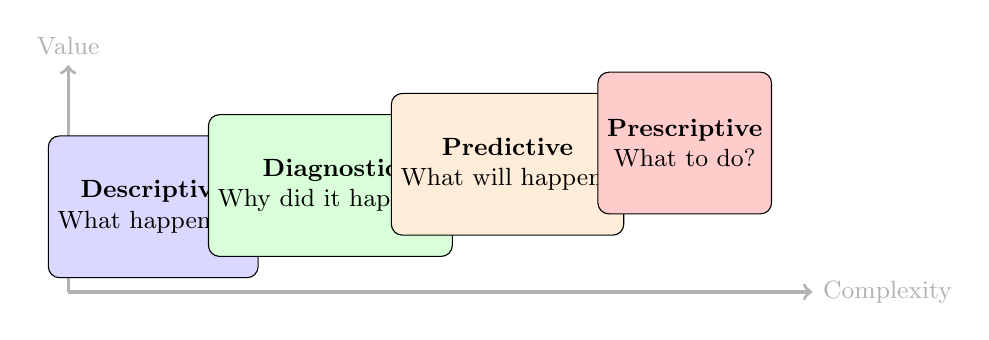
\begin{tikzpicture}[scale=0.9]
        % Arrow pointing right-up
        \draw[->, very thick, gray!60] (0,0) -- (10.5,0) node[right] {\small Complexity};
        \draw[->, very thick, gray!60] (0,0) -- (0,3.2) node[above] {\small Value};

        % Boxes
        \node[draw, fill=blue!15, minimum width=2cm, minimum height=1.8cm, rounded corners, align=center, font=\small] at (1.2,1.2) {\textbf{Descriptive}\\What happened?};
        \node[draw, fill=green!15, minimum width=2cm, minimum height=1.8cm, rounded corners, align=center, font=\small] at (3.7,1.5) {\textbf{Diagnostic}\\Why did it happen?};
        \node[draw, fill=orange!15, minimum width=2cm, minimum height=1.8cm, rounded corners, align=center, font=\small] at (6.2,1.8) {\textbf{Predictive}\\What will happen?};
        \node[draw, fill=red!20, minimum width=2cm, minimum height=1.8cm, rounded corners, align=center, font=\small] at (8.7,2.1) {\textbf{Prescriptive}\\What to do?};
    \end{tikzpicture}
    \end{center}

    \vspace{0.05cm}
    \begin{columns}
        \column{0.5\textwidth}
        \begin{itemize}\setlength{\itemsep}{0pt}
            \item \textbf{Descriptive}: dashboards, KPIs, historical reports
            \item \textbf{Diagnostic}: root-cause analysis, drill-down
        \end{itemize}
        \column{0.5\textwidth}
        \begin{itemize}\setlength{\itemsep}{0pt}
            \item \textbf{Predictive}: ML models, forecasting, RUL prediction
            \item \textbf{Prescriptive}: optimization, closed-loop control, recommendations
        \end{itemize}
    \end{columns}
\end{frame}

%==============================================================================
\section{The IoT Analytics Pipeline}
%==============================================================================

\begin{frame}{IoT Analytics Pipeline: Overview}
    \small
    \textbf{Data flows through six stages from sensor to decision:}

    \vspace{0.1cm}
    \begin{center}
    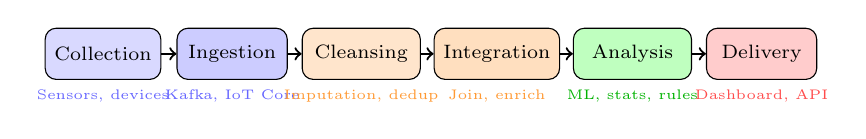
\begin{tikzpicture}[scale=0.82, every node/.style={font=\scriptsize}]
        \node[draw, fill=blue!15, minimum width=1.4cm, minimum height=0.65cm, rounded corners, align=center] (col) at (0,0) {Collection};
        \node[draw, fill=blue!20, minimum width=1.4cm, minimum height=0.65cm, rounded corners, align=center] (ing) at (2,0) {Ingestion};
        \node[draw, fill=orange!20, minimum width=1.5cm, minimum height=0.65cm, rounded corners, align=center] (cln) at (4,0) {Cleansing};
        \node[draw, fill=orange!25, minimum width=1.5cm, minimum height=0.65cm, rounded corners, align=center] (int) at (6.1,0) {Integration};
        \node[draw, fill=green!25, minimum width=1.5cm, minimum height=0.65cm, rounded corners, align=center] (ana) at (8.2,0) {Analysis};
        \node[draw, fill=red!20, minimum width=1.4cm, minimum height=0.65cm, rounded corners, align=center] (del) at (10.2,0) {Delivery};

        \draw[->, thick] (col) -- (ing);
        \draw[->, thick] (ing) -- (cln);
        \draw[->, thick] (cln) -- (int);
        \draw[->, thick] (int) -- (ana);
        \draw[->, thick] (ana) -- (del);

        \node[font=\tiny, text=blue!60] at (0,-0.65) {Sensors, devices};
        \node[font=\tiny, text=blue!60] at (2,-0.65) {Kafka, IoT Core};
        \node[font=\tiny, text=orange!80] at (4,-0.65) {Imputation, dedup};
        \node[font=\tiny, text=orange!80] at (6.1,-0.65) {Join, enrich};
        \node[font=\tiny, text=green!70!black] at (8.2,-0.65) {ML, stats, rules};
        \node[font=\tiny, text=red!70] at (10.2,-0.65) {Dashboard, API};
    \end{tikzpicture}
    \end{center}

    \vspace{0.05cm}
    \begin{columns}
        \column{0.5\textwidth}
        \begin{itemize}\setlength{\itemsep}{0pt}
            \item \textbf{Collection}: multi-source, multi-rate, multi-format
            \item \textbf{Ingestion}: single data store at scale
            \item \textbf{Cleansing}: format, validate, handle missing
        \end{itemize}
        \column{0.5\textwidth}
        \begin{itemize}\setlength{\itemsep}{0pt}
            \item \textbf{Integration}: link entities, resolve conflicts
            \item \textbf{Analysis}: ML, statistics, rules engines
            \item \textbf{Delivery}: queries, viz, real-time APIs
        \end{itemize}
    \end{columns}
\end{frame}

\begin{frame}{Data Collection and Ingestion Challenges}
    \small
    \textbf{The pipeline starts with data that is rarely clean.}

    \vspace{0.05cm}
    \begin{columns}
        \column{0.5\textwidth}
        \textbf{Collection challenges:}
        \begin{itemize}\setlength{\itemsep}{0pt}
            \item Multiple sensor types, different firmware
            \item Damaged or uncalibrated sensors
            \item Mixed protocols: MQTT, CoAP, HTTP, OPC-UA
            \item Bursty: 10k devices reconnect simultaneously
            \item Timezone and clock drift
        \end{itemize}

        \vspace{0.05cm}
        \textbf{Ingestion patterns:}
        \begin{itemize}\setlength{\itemsep}{0pt}
            \item \textbf{Batch}: Spark --- periodic load
            \item \textbf{Micro-batch}: Spark Streaming --- seconds
            \item \textbf{Stream}: Flink, Kafka --- milliseconds
        \end{itemize}

        \column{0.5\textwidth}
        \textbf{Scale:}
        \begin{itemize}\setlength{\itemsep}{0pt}
            \item Kafka: peak \textbf{605~MB/s}, p99 = 5~ms
            \item AWS IoT Core: \textbf{100B} messages/month
            \item Flink: sub-second end-to-end
        \end{itemize}

        \vspace{0.05cm}
        \begin{alertblock}{Design principle}
            Ingest first, validate later. Synchronous validation at broker scale is a bottleneck. Validate downstream in the stream processor.
        \end{alertblock}
    \end{columns}
\end{frame}

%==============================================================================
\section{Data Quality and Preprocessing}
%==============================================================================

\begin{frame}{Data Quality: The Hidden Engineering Problem}
    \small
    \textbf{A systematic review of 57 IoT publications identified 8 error types:}

    \vspace{0.05cm}
    \begin{center}
    \scriptsize
    \begin{tabular}{p{3cm}p{3cm}p{5.5cm}}
        \toprule
        \textbf{Error type} & \textbf{Frequency} & \textbf{Example / Impact} \\
        \midrule
        Outliers & Most common & Sensor spike: 200°C from a 25°C sensor \\
        Missing data & Very common & 5--70\% missing rates in real deployments \\
        Bias / offset & Common & Sensor reads 2°C too high consistently \\
        Drift & Common & Gradual deviation due to material aging \\
        Noise & Common & Random fluctuation around true value \\
        Constant / stuck & Moderate & Sensor locked at last value after fault \\
        Uncertainty & Moderate & Calibration tolerance not modeled \\
        Stuck-at-zero & Less common & Division-by-zero or reset condition \\
        \bottomrule
    \end{tabular}
    \end{center}

    \begin{alertblock}{Sensor drift is irreversible}
        Unlike noise (filterable) or outliers (detectable), drift is a gradual, permanent deviation. ML-based calibration using XGBoost achieves R\textsuperscript{2} of 0.86--0.92 for PM2.5 correction.
    \end{alertblock}
\end{frame}

\begin{frame}{Preprocessing Pipeline}
    \small
    \textbf{Standard preprocessing sequence for IoT sensor data:}

    \vspace{0.05cm}
    \begin{center}
    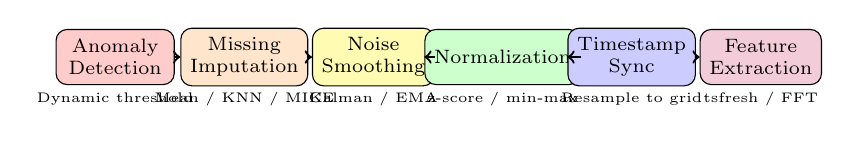
\begin{tikzpicture}[scale=0.82, every node/.style={font=\scriptsize}]
        \node[draw, fill=red!20, minimum width=1.5cm, minimum height=0.7cm, rounded corners, align=center] (n0) at (0,0) {Anomaly\\Detection};
        \node[font=\tiny, align=center] at (0,-0.65) {Dynamic threshold};
        \node[draw, fill=orange!20, minimum width=1.5cm, minimum height=0.7cm, rounded corners, align=center] (n1) at (2,0) {Missing\\Imputation};
        \node[font=\tiny, align=center] at (2,-0.65) {Mean / KNN / MICE};
        \node[draw, fill=yellow!30, minimum width=1.5cm, minimum height=0.7cm, rounded corners, align=center] (n2) at (4,0) {Noise\\Smoothing};
        \node[font=\tiny, align=center] at (4,-0.65) {Kalman / EMA};
        \node[draw, fill=green!20, minimum width=1.5cm, minimum height=0.7cm, rounded corners, align=center] (n3) at (6,0) {Normalization};
        \node[font=\tiny, align=center] at (6,-0.65) {z-score / min-max};
        \node[draw, fill=blue!20, minimum width=1.5cm, minimum height=0.7cm, rounded corners, align=center] (n4) at (8,0) {Timestamp\\Sync};
        \node[font=\tiny, align=center] at (8,-0.65) {Resample to grid};
        \node[draw, fill=purple!20, minimum width=1.5cm, minimum height=0.7cm, rounded corners, align=center] (n5) at (10,0) {Feature\\Extraction};
        \node[font=\tiny, align=center] at (10,-0.65) {tsfresh / FFT};
        \draw[->, thick] (n0) -- (n1);
        \draw[->, thick] (n1) -- (n2);
        \draw[->, thick] (n2) -- (n3);
        \draw[->, thick] (n3) -- (n4);
        \draw[->, thick] (n4) -- (n5);
    \end{tikzpicture}
    \end{center}

    \vspace{0.05cm}
    \begin{columns}
        \column{0.5\textwidth}
        \textbf{Missing data strategies:}
        \begin{itemize}\setlength{\itemsep}{0pt}
            \item \textbf{Forward fill}: use last known value (common for slow sensors)
            \item \textbf{Interpolation}: linear or spline for smooth signals
            \item \textbf{MICE}: multivariate imputation by chained equations
            \item \textbf{ML imputation}: KNN, Random Forest-based
        \end{itemize}

        \column{0.5\textwidth}
        \textbf{Anomaly detection (preprocessing stage):}
        \begin{itemize}\setlength{\itemsep}{0pt}
            \item Dynamic threshold: $\mu \pm k\sigma$ per rolling window
            \item IQR-based: flag values outside $Q1 - 1.5\cdot IQR$
            \item Isolation Forest: unsupervised, fast
            \item \textbf{Rule}: do not impute flagged outliers --- mark and exclude
        \end{itemize}
    \end{columns}
\end{frame}

%==============================================================================
\section{Feature Engineering for IoT}
%==============================================================================

\begin{frame}{Time-Series Feature Engineering}
    \small
    \textbf{Raw sensor values are rarely the right ML input. Features are.}

    \vspace{0.05cm}
    \begin{columns}
        \column{0.5\textwidth}
        \textbf{Statistical features (per window):}
        \begin{itemize}\setlength{\itemsep}{0pt}
            \item Mean, std, min, max, range
            \item Skewness, kurtosis
            \item Percentiles: P5, P50, P95, P99
            \item Zero-crossing rate, autocorrelation
        \end{itemize}

        \vspace{0.05cm}
        \textbf{Frequency-domain features:}
        \begin{itemize}\setlength{\itemsep}{0pt}
            \item \textbf{FFT}: dominant frequency, spectral centroid
            \item \textbf{PSD}: energy per frequency band
            \item \textbf{STFT}: time-frequency for non-stationary signals
            \item Bearing faults appear at specific FFT frequencies
        \end{itemize}

        \column{0.5\textwidth}
        \textbf{Windowing strategies:}
        \begin{itemize}\setlength{\itemsep}{0pt}
            \item \textbf{Tumbling}: non-overlapping, each sample used once
            \item \textbf{Sliding}: overlapping, richer context, more data
            \item \textbf{Session}: event-triggered, variable-length
        \end{itemize}

        \vspace{0.05cm}
        \textbf{Automated feature extraction:}
        \begin{itemize}\setlength{\itemsep}{0pt}
            \item \textbf{tsfresh}: 787 features, automated selection
            \item \textbf{Catch22}: 22 canonical, interpretable
            \item \textbf{ROCKET}: 10k random kernels, SOTA classification
        \end{itemize}
    \end{columns}
\end{frame}

%==============================================================================
\section{ML Fundamentals for IoT}
%==============================================================================

\begin{frame}{What Is a Machine Learning Model?}
    \scriptsize
    \textbf{A model is a mathematical function that maps inputs to outputs --- learned automatically from data.}

    \vspace{0.03cm}
    \begin{columns}
        \column{0.5\textwidth}
        \textbf{You already know this concept:}
        \begin{itemize}\setlength{\itemsep}{0pt}
            \item Linear regression fits a line $y = mx + b$ to data
            \item You choose $m$ and $b$ to minimize the error between predictions and real values
            \item \textbf{ML generalizes this}: fit any function (not just a line) to any number of inputs
        \end{itemize}

        \vspace{0.03cm}
        \textbf{In IoT terms:}
        \begin{itemize}\setlength{\itemsep}{0pt}
            \item \textbf{Input}: sensor readings (temperature, vibration, current\ldots)
            \item \textbf{Output}: a decision (``fault'', ``RUL = 12 days'', ``anomaly score = 0.93'')
            \item \textbf{Training}: finding the best function using historical labeled data
        \end{itemize}

        \column{0.5\textwidth}
        \textbf{Three problem types:}
        \begin{itemize}\setlength{\itemsep}{0pt}
            \item \textbf{Classification}: assign a label\\{``Is this bearing fault A, B, or normal?''}
            \item \textbf{Regression}: predict a number\\{``How many days until failure?''}
            \item \textbf{Anomaly detection}: flag unusual patterns\\{``This reading does not look like normal operation''}
        \end{itemize}

        \vspace{0.03cm}
        \begin{alertblock}{Key intuition}
            Training = automated curve fitting on historical data. Inference = applying that curve to new data.
        \end{alertblock}
    \end{columns}
\end{frame}

\begin{frame}{Training, Validation, and the Bias-Variance Tradeoff}
    \scriptsize
    \textbf{How do we know if a model is good --- or just memorizing the training data?}

    \vspace{0.03cm}
    \begin{columns}
        \column{0.5\textwidth}
        \textbf{The three-split workflow:}
        \begin{itemize}\setlength{\itemsep}{0pt}
            \item \textbf{Training set} (70\%): the model learns from this data
            \item \textbf{Validation set} (15\%): tune hyperparameters, detect overfitting
            \item \textbf{Test set} (15\%): final honest evaluation --- touch it only once
        \end{itemize}

        \vspace{0.03cm}
        \textbf{Overfitting vs.\ underfitting:}
        \begin{itemize}\setlength{\itemsep}{0pt}
            \item \textbf{Underfitting}: model too simple, misses real patterns (high bias)
            \item \textbf{Overfitting}: memorizes training noise, fails on new data (high variance)
            \item \textbf{Goal}: generalization --- good performance on unseen data
        \end{itemize}

        \column{0.5\textwidth}
        \textbf{IoT-specific complication:}
        \begin{itemize}\setlength{\itemsep}{0pt}
            \item Time-series is \textbf{not i.i.d.} --- tomorrow depends on today
            \item Never shuffle randomly! Use \textbf{walk-forward validation}: train on past, test on future
            \item Otherwise the model ``cheats'' by seeing future data during training
        \end{itemize}

        \vspace{0.03cm}
        \begin{exampleblock}{Evaluation metrics}
            \textbf{Classification}: accuracy, precision, recall, F1-score\\
            \textbf{Regression}: MAE, RMSE\\
            \textbf{Anomaly}: precision-recall AUC\\
            (Never use accuracy alone on imbalanced IoT data)
        \end{exampleblock}
    \end{columns}
\end{frame}

\begin{frame}{Why Neural Networks? From Regression to Deep Learning}
    \scriptsize
    \textbf{Neural networks extend linear regression to capture complex, non-linear patterns in sensor data.}

    \vspace{0.05cm}
    \begin{columns}
        \column{0.48\textwidth}
        \textbf{From regression to a neural network:}
        \begin{itemize}\setlength{\itemsep}{1pt}
            \item Linear regression: $\hat{y} = w_1 x_1 + w_2 x_2 + b$
            \item Add a non-linear activation (e.g.\ ReLU): $f(z) = \max(0, z)$
            \item Stack layers: each layer transforms the input, learning richer representations
            \item \textbf{Training}: gradient descent adjusts weights $w$ to minimize prediction error
        \end{itemize}

        \vspace{0.03cm}
        \textbf{Why do we need this for IoT?}
        \begin{itemize}\setlength{\itemsep}{1pt}
            \item Bearing faults are \textbf{not linearly separable} from normal operation in raw sensor space
            \item A neural network learns the non-linear boundary automatically
            \item Classical regression would require hand-crafted features for each fault type
        \end{itemize}

        \column{0.52\textwidth}
        \textbf{Architectures used in this module:}
        \begin{itemize}\setlength{\itemsep}{1pt}
            \item \textbf{Random Forest}: many decision trees voting together --- robust, interpretable, no gradient needed
            \item \textbf{LSTM} (Long Short-Term Memory): a network with memory --- processes sequences, remembers past readings. Ideal for time-series
            \item \textbf{CNN} (Convolutional): applies sliding filters to detect local patterns (e.g.\ frequency peaks in FFT)
            \item \textbf{Autoencoder}: network trained to compress and reconstruct normal data --- anomalies fail reconstruction
        \end{itemize}

        \vspace{0.03cm}
        \begin{alertblock}{No math required today}
            You do not need to derive backpropagation. You need to understand \textbf{what each architecture is good at} and \textbf{why}.
        \end{alertblock}
    \end{columns}
\end{frame}

%==============================================================================
\section{ML Algorithms for IoT}
%==============================================================================

\begin{frame}{ML for IoT: Algorithm Selection}
    \small
    \textbf{Match the algorithm to the problem type:}

    \vspace{0.03cm}
    \begin{center}
    \tiny
    \begin{tabular}{p{2.3cm}p{2.8cm}p{3cm}p{3cm}}
        \toprule
        \textbf{Problem} & \textbf{Algorithm} & \textbf{Strengths} & \textbf{IoT use case} \\
        \midrule
        Classification & Random Forest & Noise robust, interpretable & Fault type classification \\
        Classification & XGBoost / LightGBM & Best tabular accuracy & Equipment health scoring \\
        Regression & LSTM, BiLSTM & Temporal dependencies & RUL prediction, energy forecast \\
        Regression & CNN-LSTM+Attention & Spatial + temporal & State-of-the-art PdM \\
        Anomaly (unsupervised) & Autoencoder & No labels needed & Novelty detection \\
        Anomaly (unsupervised) & Isolation Forest & Fast, scalable & Real-time streaming \\
        Time-series forecast & Prophet & Seasonality, trends & Energy demand forecasting \\
        Time-series forecast & TimeFM / Chronos & Zero-shot, foundation model & New deployments (2025--2026) \\
        \bottomrule
    \end{tabular}
    \end{center}

    \begin{alertblock}{Practical rule}
        Start with XGBoost on engineered features. If accuracy is insufficient, move to deep learning. Deep learning without sufficient data ($<$10k labeled samples) rarely wins.
    \end{alertblock}
\end{frame}

\begin{frame}{Predictive Maintenance: The Flagship Application}
    \small
    \textbf{PdM}: predict equipment failure before it happens, from continuous telemetry.

    \vspace{0.05cm}
    \begin{columns}
        \column{0.5\textwidth}
        \textbf{Data pipeline:}
        \begin{itemize}\setlength{\itemsep}{0pt}
            \item Vibration (10--50~kHz), temp, current, pressure
            \item MQTT/OPC-UA $\rightarrow$ Kafka $\rightarrow$ feature store
            \item Sliding window $\rightarrow$ RUL prediction
        \end{itemize}

        \vspace{0.05cm}
        \textbf{SOTA architecture (2026):}
        \begin{itemize}\setlength{\itemsep}{0pt}
            \item CNN: spatial features from vibration FFT
            \item LSTM: temporal degradation trend
            \item Attention: weights relevant time steps
            \item RMSE 11.5--14.5 cycles on NASA C-MAPSS
        \end{itemize}

        \column{0.5\textwidth}
        \textbf{Benchmark datasets:}
        \begin{itemize}\setlength{\itemsep}{0pt}
            \item \textbf{NASA C-MAPSS}: turbofan, 21 sensors, 4 scenarios, 1,000+ papers
            \item \textbf{CWRU Bearing}: 12/48~kHz, single-point faults, de facto standard
            \item \textbf{FEMTO}: accelerated degradation, IEEE PHM
        \end{itemize}

        \vspace{0.05cm}
        \begin{exampleblock}{Real impact}
            PdM: \textbf{40\%} cost reduction, \textbf{50\%} less downtime (McKinsey). EUROGATE: >92\% fault accuracy.
        \end{exampleblock}
    \end{columns}
\end{frame}

\begin{frame}{Anomaly Detection for IoT}
    \small
    \textbf{In IoT, ``normal'' is abundant. Faults are rare ($<$1\% of data). No labels available.}

    \vspace{0.05cm}
    \begin{columns}
        \column{0.5\textwidth}
        \textbf{Unsupervised approaches:}
        \begin{itemize}\setlength{\itemsep}{0pt}
            \item \textbf{Autoencoder}: train on normal data; high reconstruction error = anomaly. 100\% recall, >90\% precision on IoT datasets (PMC 2024)
            \item \textbf{Isolation Forest}: random partitioning; anomalies isolated in fewer splits
            \item \textbf{LOF}: local outlier factor; density-based
            \item \textbf{LSTM-based}: predict next step; large prediction error = anomaly
        \end{itemize}

        \column{0.5\textwidth}
        \textbf{Deep learning approaches (2024--2026):}
        \begin{itemize}\setlength{\itemsep}{0pt}
            \item \textbf{DCDetector} (KDD 2023): dual-attention contrastive learning for multivariate time-series
            \item \textbf{CAE-T}: CNN autoencoder + transformer for ICS monitoring
            \item \textbf{PatchTST}: patch-based transformer, SOTA on several benchmarks
        \end{itemize}

        \vspace{0.05cm}
        \begin{alertblock}{Class imbalance warning}
            A model that classifies everything as ``normal'' gets 99\% accuracy on a dataset with 1\% faults. Use F1-score, precision-recall, and ROC-AUC --- never just accuracy.
        \end{alertblock}
    \end{columns}
\end{frame}

%==============================================================================
\section{Stream Analytics}
%==============================================================================

\begin{frame}{Stream Analytics: Real-Time Intelligence}
    \small
    \textbf{Analytics at the speed of data --- not in batch, but as it arrives.}

    \vspace{0.05cm}
    \begin{columns}
        \column{0.5\textwidth}
        \textbf{Apache Flink:}
        \begin{itemize}\setlength{\itemsep}{0pt}
            \item True streaming (not micro-batch)
            \item Stateful computation over event time
            \item Watermarks for out-of-order events
            \item Exactly-once semantics + checkpointing
            \item Latency: sub-100~ms end-to-end
        \end{itemize}

        \vspace{0.05cm}
        \textbf{Spark Structured Streaming:}
        \begin{itemize}\setlength{\itemsep}{0pt}
            \item Micro-batch: 100~ms--1~s windows
            \item Same DataFrame API as batch Spark
            \item Delta Lake integration for streaming upserts
        \end{itemize}

        \column{0.5\textwidth}
        \textbf{Kafka Streams / ksqlDB:}
        \begin{itemize}\setlength{\itemsep}{0pt}
            \item SQL-like streaming queries
            \item Embed ML models as UDFs
            \item No separate cluster: runs inside Kafka
        \end{itemize}

        \vspace{0.05cm}
        \begin{exampleblock}{Production pattern}
            ksqlDB UDF: embed XGBoost as Java UDF in Kafka. Every MQTT message scored in $<$5~ms, no data leaving the bus.
        \end{exampleblock}
    \end{columns}
\end{frame}

\begin{frame}{Windowing in Stream Analytics}
    \small
    \textbf{All stream analytics reduce to: apply a function over a window of data.}

    \vspace{0.05cm}
    \begin{center}
    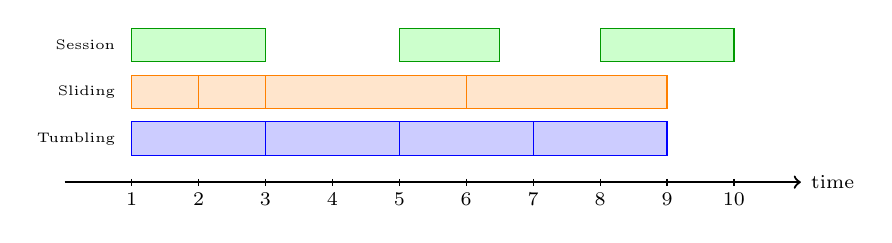
\begin{tikzpicture}[scale=0.85, every node/.style={font=\scriptsize}]
        % Timeline
        \draw[->, thick] (0,0) -- (11,0) node[right] {time};
        \foreach \x in {1,2,3,4,5,6,7,8,9,10} {
            \draw (\x,0.05) -- (\x,-0.05);
            \node at (\x,-0.25) {\x};
        }

        % Tumbling windows
        \draw[fill=blue!20, draw=blue] (1,0.4) rectangle (3,0.9);
        \draw[fill=blue!20, draw=blue] (3,0.4) rectangle (5,0.9);
        \draw[fill=blue!20, draw=blue] (5,0.4) rectangle (7,0.9);
        \draw[fill=blue!20, draw=blue] (7,0.4) rectangle (9,0.9);
        \node[left, font=\tiny] at (0.9,0.65) {Tumbling};

        % Sliding windows
        \draw[fill=orange!20, draw=orange] (1,1.1) rectangle (4,1.6);
        \draw[fill=orange!20, draw=orange] (2,1.1) rectangle (5,1.6);
        \draw[fill=orange!20, draw=orange] (3,1.1) rectangle (6,1.6);
        \draw[fill=orange!20, draw=orange] (6,1.1) rectangle (9,1.6);
        \node[left, font=\tiny] at (0.9,1.35) {Sliding};

        % Session windows
        \draw[fill=green!20, draw=green!60!black] (1,1.8) rectangle (3,2.3);
        \draw[fill=green!20, draw=green!60!black] (5,1.8) rectangle (6.5,2.3);
        \draw[fill=green!20, draw=green!60!black] (8,1.8) rectangle (10,2.3);
        \node[left, font=\tiny] at (0.9,2.05) {Session};
    \end{tikzpicture}
    \end{center}

    \vspace{0.02cm}
    \begin{columns}
        \column{0.33\textwidth}
        \textbf{Tumbling:} Fixed, non-overlapping. Hourly summaries.

        \column{0.33\textwidth}
        \textbf{Sliding:} Overlapping, richer context. Anomaly detection.

        \column{0.33\textwidth}
        \textbf{Session:} Event-triggered, variable. User activity tracking.
    \end{columns}
\end{frame}

%==============================================================================
\section{Analytics Tools and Platforms}
%==============================================================================

\begin{frame}{Big Data Analytics Tools (2026)}
    \small
    \textbf{The ecosystem has consolidated around a few dominant platforms:}

    \vspace{0.05cm}
    \begin{center}
    \scriptsize
    \begin{tabular}{p{2.3cm}p{2.5cm}p{2.5cm}p{2.5cm}p{1.8cm}}
        \toprule
        \textbf{Tool} & \textbf{Data types} & \textbf{Pipeline stages} & \textbf{Algorithms} & \textbf{License} \\
        \midrule
        \textbf{Apache Spark} & Structured + unstructured & Ingest, clean, integrate, analyze & MLlib, DL via TF/PT & Open source \\
        \textbf{Apache Flink} & Streaming + batch & Ingest, clean, analyze (real-time) & Flink ML, CEP & Open source \\
        \textbf{Databricks} & All types & Full pipeline & MLflow, AutoML & Commercial \\
        \textbf{AWS EMR/Glue} & All types & Full pipeline & SageMaker integration & Managed \\
        \textbf{DuckDB} & Parquet, CSV, JSON & Query, analyze & SQL, Python UDFs & Open source \\
        \textbf{Oracle / PostgreSQL} & Structured & Query, analyze & Oracle ML, extensions & Mixed \\
        \bottomrule
    \end{tabular}
    \end{center}

    \begin{exampleblock}{2026 trend: DuckDB for IoT analytics}
        Query years of Parquet files on S3 directly from a Python notebook. No cluster, no ETL, no cost beyond S3. For exploratory analytics on IoT cold storage, DuckDB is the 2026 answer.
    \end{exampleblock}
\end{frame}

\begin{frame}{Visualization and Delivery}
    \small
    \textbf{Analytics value is realized only when insights reach decision-makers.}

    \vspace{0.05cm}
    \begin{columns}
        \column{0.5\textwidth}
        \textbf{Real-time dashboards:}
        \begin{itemize}\setlength{\itemsep}{0pt}
            \item \textbf{Grafana}: open-source, InfluxDB/Prometheus native
            \item \textbf{Kibana}: OpenSearch, log analytics
            \item \textbf{Power BI / Tableau}: business BI + real-time
            \item \textbf{Custom}: React + WebSocket, sub-second
        \end{itemize}

        \vspace{0.05cm}
        \textbf{Alerting:}
        \begin{itemize}\setlength{\itemsep}{0pt}
            \item Grafana: threshold + ML-based alerts
            \item PagerDuty / OpsGenie: on-call routing
            \item \textbf{SLO-based}: alert on error budget burn rate
        \end{itemize}

        \column{0.5\textwidth}
        \textbf{ML model serving:}
        \begin{itemize}\setlength{\itemsep}{0pt}
            \item \textbf{REST API}: FastAPI + Docker, on-demand
            \item \textbf{KServe}: Kubernetes-native, autoscaling
            \item \textbf{ONNX Runtime}: same model, edge + cloud
            \item \textbf{Edge}: TFLite, Edge Impulse for MCU
        \end{itemize}

        \vspace{0.05cm}
        \begin{alertblock}{Latency contract}
            $<$10~ms: edge. $<$100~ms: co-located API. $<$1~s: cloud API. $>$1~s: async pipeline. Define SLA first.
        \end{alertblock}
    \end{columns}
\end{frame}

%==============================================================================
\section{Advanced Analytics Topics}
%==============================================================================

\begin{frame}{Digital Twins: Analytics at the System Level}
    \small
    \textbf{A digital twin synchronizes a virtual model with a physical asset via continuous IoT data.}

    \vspace{0.05cm}
    \begin{columns}
        \column{0.5\textwidth}
        \textbf{AWS 4-level maturity model:}
        \begin{itemize}\setlength{\itemsep}{0pt}
            \item \textbf{L1 Descriptive}: 3D visualization, static data
            \item \textbf{L2 Informative}: enriched with real-time IoT streams
            \item \textbf{L3 Predictive}: ML-based forecasting, failure prediction
            \item \textbf{L4 Living}: closed-loop, autonomous adaptation
        \end{itemize}

        \vspace{0.05cm}
        \textbf{Hybrid physics-ML twins (2026):}
        \begin{itemize}\setlength{\itemsep}{0pt}
            \item Physics model handles known failure modes
            \item ML catches deviations from expected behavior
            \item Self-calibrating: drift correction from live data
        \end{itemize}

        \column{0.5\textwidth}
        \textbf{Business impact:}
        \begin{itemize}\setlength{\itemsep}{0pt}
            \item Manufacturing press: 87\% accuracy, failures predicted 5--8 days ahead
            \item Unplanned downtime reduced by \textbf{62\%}
            \item Component life extended from 3,000 to 4,200 cycles
            \item Digital twin market: \textbf{\$13.6B in 2024} $\rightarrow$ \$428B by 2034
        \end{itemize}

        \vspace{0.05cm}
        \begin{exampleblock}{Platforms}
            Azure Digital Twins (DTDL v3), AWS IoT TwinMaker, Siemens Xcelerator + NVIDIA Omniverse. All integrate directly with IoT Hub / IoT Core for live data sync.
        \end{exampleblock}
    \end{columns}
\end{frame}

\begin{frame}{Time-Series Foundation Models (2025--2026)}
    \small
    \textbf{Biggest recent shift: pre-trained models that work zero-shot on new IoT data.}

    \vspace{0.05cm}
    \begin{columns}
        \column{0.5\textwidth}
        \textbf{Why they matter:}
        \begin{itemize}\setlength{\itemsep}{0pt}
            \item Labeling IoT data: expensive and slow
            \item New deployments: no historical data yet
            \item Foundation models: deploy and forecast immediately
        \end{itemize}

        \vspace{0.05cm}
        \textbf{Key models (2024--2026):}
        \begin{itemize}\setlength{\itemsep}{0pt}
            \item \textbf{Chronos} (Amazon): zero-shot matches fine-tuned on 42 datasets
            \item \textbf{TimesFM} (Google): \textbf{16$\times$ faster} than fine-tuning
            \item \textbf{MOMENT} (CMU): open-source, F1 0.85 zero-shot
            \item \textbf{MOIRAI} (Salesforce): 27B+ observations
        \end{itemize}

        \column{0.5\textwidth}
        \textbf{How to use them:}
        \begin{itemize}\setlength{\itemsep}{0pt}
            \item Provide recent context window
            \item Model forecasts next N steps --- no training
            \item Fine-tune with small labeled set if needed
        \end{itemize}

        \vspace{0.05cm}
        \begin{alertblock}{2026 practical guidance}
            No labels $\rightarrow$ Chronos/TimesFM zero-shot.\\Industrial signals $\rightarrow$ 3--6 months + fine-tune.\\Anomaly only $\rightarrow$ autoencoder on normal data.
        \end{alertblock}
    \end{columns}
\end{frame}

%==============================================================================
\section{Analytics at Scale: Challenges}
%==============================================================================

\begin{frame}{Distributed Analytics Challenges}
    \small
    \textbf{Analytics at IoT scale introduces problems absent from lab settings.}

    \vspace{0.05cm}
    \begin{columns}
        \column{0.5\textwidth}
        \textbf{Decentralized processing:}
        \begin{itemize}\setlength{\itemsep}{0pt}
            \item Cannot centralize all data: bandwidth + cost
            \item \textbf{MapReduce}: split and aggregate
            \item \textbf{Federated learning}: train locally, share weights
            \item \textbf{Edge inference}: model runs where data is
        \end{itemize}

        \vspace{0.05cm}
        \textbf{Security and privacy:}
        \begin{itemize}\setlength{\itemsep}{0pt}
            \item GDPR: wearables/smart home data jurisdiction rules
            \item HIPAA: encryption + audit trail mandatory
            \item FGSM: most common adversarial attack
            \item NIST AI 100-2e2025: adversarial ML taxonomy
        \end{itemize}

        \column{0.5\textwidth}
        \textbf{Model interpretability:}
        \begin{itemize}\setlength{\itemsep}{0pt}
            \item Black-box = unacceptable in safety-critical IoT
            \item \textbf{SHAP}: explain any prediction
            \item \textbf{LIME}: local linear approximations
            \item \textbf{Attention maps}: which time steps matter
        \end{itemize}

        \vspace{0.05cm}
        \begin{exampleblock}{Speed vs.\ accuracy}
            Stream + edge = fast but approximate. Batch + cloud = slow but accurate. Design decision. Define SLA first.
        \end{exampleblock}
    \end{columns}
\end{frame}

%==============================================================================
\section{Summary}
%==============================================================================

\begin{frame}{Key Takeaways}
    \scriptsize
    \begin{columns}
        \column{0.5\textwidth}
        \textbf{Fundamentals:}
        \begin{itemize}\setlength{\itemsep}{0pt}
            \item 4 types: descriptive $\rightarrow$ prescriptive
            \item Pipeline: collect $\rightarrow$ ingest $\rightarrow$ clean $\rightarrow$ analyze $\rightarrow$ deliver
            \item 8 sensor error types; 5--70\% missing data
            \item Feature engineering bridges sensor to ML
        \end{itemize}

        \vspace{0.03cm}
        \textbf{Algorithms:}
        \begin{itemize}\setlength{\itemsep}{0pt}
            \item XGBoost: tabular + engineered features
            \item CNN-LSTM-Attention: SOTA PdM/RUL
            \item Autoencoder: anomaly, no labels needed
            \item Chronos/TimesFM: zero-shot foundation models
        \end{itemize}

        \column{0.5\textwidth}
        \textbf{Tools:}
        \begin{itemize}\setlength{\itemsep}{0pt}
            \item Kafka + Flink: real-time stream analytics
            \item Spark: batch and micro-batch at scale
            \item DuckDB: ad-hoc on S3 Parquet
        \end{itemize}

        \vspace{0.03cm}
        \textbf{2026 trends:}
        \begin{itemize}\setlength{\itemsep}{0pt}
            \item Foundation models: zero-shot forecasting
            \item Digital twins: L4 living, closed-loop
            \item Federated learning + DuckDB + Iceberg
        \end{itemize}
    \end{columns}
    \begin{alertblock}{The Core Lesson}
        Collect data. Few extract value. The difference: end-to-end analytics pipeline from day one.
    \end{alertblock}
\end{frame}

\begin{frame}{Questions?}
    \begin{center}
        \Huge Questions?

        \vspace{0.8cm}
        \normalsize
        \textbf{Eduardo Baena}\\
        \texttt{e.baena@northeastern.edu}\\[0.3cm]
        \textit{Next: Module 9 --- AI/MLOps for IoT}
    \end{center}
\end{frame}

\end{document}
